\chapter{Gaseous initial conditions for JICF}
\label{app:gas_initial_cond_JICF}





\section*{Injection of synthetic turbulence}
\label{subsec:ch5_inflow_conditions_synthetic_turbulence}

% References for turbulence injection
% https://www.cfd-online.com/Wiki/Turbulence_length_scale
% https://www.cfd-online.com/Wiki/Turbulence_intensity
% https://www.simscale.com/forum/t/defining-turbulent-boundary-conditions/80895

Prescription of inlet velocity profiles should take into account the contribution of large energy-containing eddies. For this purpose, fluctuations can be added to the mean profiles by specifying either their energy spectrum or their characteristic length scales and their magnitude. These fluctuating components can be obtained by several means. One of the first methods developed consisted of using periodic boundary conditions to reintroduce the outlet velocity field at the inlet in DNS simulations of channels \citemColor[spalart_direct_1988,liu_interaction_1996]. Such methods rely either on the presence of self-similarity in the channels, which does not always occur, or on adding a forcing term at the outlet to reconvert the boundary layer thickness to its value upstream for reintroducing it into the inlet. To circumvent these issues, the recycling method was proposed by \citeColor[lund_generation_1998]. This technique consists of obtaining the turbulent data at several planes downstream the inlet, compare the velocity fields and correct the inlet conditions accordingly to match the desired data. Recycling methods have been extended and can be divided in weak and strong methods. Other families of techniques include the generation of synthetic turbulence by for superposition of sinusoidal waves \citemColor[kraichnan_diffusion_1970,batten_interfacing_2004] or by moments' determination \citepColor[pamies_generation_2009]. A review of these and other turbulence generation methodologies can be found in \citeColor[wu_inflow_2017].

In this work, homogeneous synthetic turbulence is injected through the inlet by specifying the integral length scale of the flow $L_T$ and the fluctuating velocity components $u'$. Since experimental data on the fluctuating field for the configuration of \citepColor[becker_breakup_2002] is not available, both magnitudes are estimated with the following formulas \citepColor[ansys_ansys_2018]:
% [1] ANSYS, Inc. (2018), "ANSYS Fluent User's Guide, Release 19.0", Equation (6.68). 

\begin{equation}
u' \approx I u_g  ~~~~ ; ~~~~ L_t \approx 0.07 D_h
\end{equation}

where $I$ is the turbulent intensity can be obtained from the following correlation:

\begin{equation}
I = 0.16 Re_g^{-1/8}
\end{equation}

For each operating point shown in Table \ref{tab:jicf_operating_conditions}, the estimated parameters for specifying turbulent profiles are shown in Table \ref{tab:jicf_operating_conditions_turbulent_injection_parameters}.


\section*{Characteristic flow-through time}

With the inlet velocity specified with a mean profile and turbulence fluctuations, gaseous simulations can be run to generate initial conditions for the liquid simulations. The initial solution needs to be an established velocity profile where the mean and rms values of velocity components are converged. To get an idea of the flow establishment, the flow-through time in the channel $\tau_\mathrm{ft}$ is defined:

\begin{equation}
\tau_\mathrm{ft} = \frac{L}{u_g}
\end{equation}

where $L = 120$ mm is the distance from the gaseous inlet to the liquid injector (see Figure \ref{fig:numerical_setup_maquette_JICF_DLR}). This quantity represents the time that a gas particle takes, in average, to reach the liquid injector location from the inlet of the domain. Flow-through times for each operating point are shown in Table \ref{tab:jicf_operating_conditions_turbulent_injection_parameters}.

\begin{table}[!h]
\centering
\caption{Parameters characterising inflow turbulent fields and flow-through time $\tau_\mathrm{ft}$ in JICF simulations}
\begin{tabular}{ccccc}
\thickhline
\textbf{Operating point} &  $L_t$ [mm] &  $I$ [\%] & $u'$ [m s$^{-1}$] & $\tau_\mathrm{ft}$ [ms] \\ %
\thickhline
Low Weber & 3 & 2.88 & 2.5 & 1.6 \\
%\hline
High Weber & 3 & 2.78 & 3.0 & 1.2  \\
\thickhline
\end{tabular}
\label{tab:jicf_operating_conditions_turbulent_injection_parameters}
\end{table}


\section*{Mesh independence study with high Weber operating point}

In first place, a mesh independence study has been performed with single-phase simulations (without fuel injection) to capture correctly the gaseous turbulent features that can affect the liquid field. For this purpose, 3 grids are tested with the high Weber operating condition. The inlet velocity profile includes the mean velocity profile and the turbulence fluctuations as defined in Table \ref{tab:jicf_operating_conditions_turbulent_injection_parameters}. The meshes differ in the baseline cell size at the region upstream the liquid injection nozzle, which measures $120$ mm (see Figure \ref{fig:numerical_setup_maquette_JICF_DLR}). This is the region of interest for turbulence development, since it is the gaseous field upstream the injection nozzle the one that will affect the liquid jet. Three meshes are used with baseline mesh sizes of values $\Delta x_\mathrm{ups} = 1, ~0.5, ~0.3$ mm, summarized in Table \ref{tab:jicf_mesh_independence_gaseous_study}. The three refinement levels tested in this section are shown in Figure \ref{fig:ics_mesh_independency_study_up_meshes}, where a magnified view of the red rectangle from Figure \ref{fig:jicf_dlr_mesh} is displayed. The mesh elsewhere is not refined and maintained to the values given previously in $\S$\ref{sec:computational_setup}. %The mesh shown in Figure \ref{fig:jicf_dlr_mesh} is the chosen grid with baseline cell size upstream the injector $\Delta x_\mathrm{ups} = 0.5$ mm.

\begin{table}[!h]
\centering
\caption{Configurations tested for the mesh independence study}
\begin{tabular}{cccccc}
\thickhline
Mesh & $\Delta x_\mathrm{ups}$ [mm] &  $\#$ elements & $\#$ nodes \\ %& Minimum cell size $\Delta x$ [$\mu$m]\\ %
\thickhline
Coarse & 1.0 & 59,664,589 & 10,510,540 \\
%\hline
Fine & 0.5 & 66,264,433 & 11,641,585 \\
%\hline
Very fine & 0.3 & 94,192,955 & 17,155,591 \\
\thickhline
\end{tabular}
\label{tab:jicf_mesh_independence_gaseous_study}
\end{table}

\begin{figure}[ht]
\centering
\includeinkscape[inkscapelatex=false,scale=0.75]{./part2_developments/figures_ch5_resolved_JICF/results_ics_mesh_convergence_mesh_and_up/meshes}
\caption[Baseline meshes in the region spanning from the inlet to the nozzle injector]{Baseline meshes in the region spanning from the inlet to the nozzle injector. Zoom-in the red rectangle of Figure \ref{fig:jicf_dlr_mesh}. From left to right: $\Delta x_\mathrm{ups} = 1, 0.5, 0.3$ mm.}
\label{fig:ics_mesh_independency_study_up_meshes}
\end{figure}


A total of four simulations have been performed: one simulation per mesh with the imposed turbulent fluctuations at the inlet, and one without injecting synthetic turbulence for the resolution $\Delta x_\mathrm{ups} = 0.5$ mm. For flow establishment, the simulations are firstly run for a total physical time of 6 times the flow-through time, i.e. 7.2 ms. From this stage on, statistics are collected. To check the convergence of the simulations, the mean axial velocity $u$ and mean Turbulent Kinetic Energy (TKE) have been integrated along a vertical line upstream the injection point in the middle plane of the domain, shown in Figure \ref{fig:ics_mesh_independency_study_up_fields} right. These line-integrated magnitudes can be defined as follows:


\begin{equation}
\label{eq:line_averaged_u_and_TKE}
\langle u \rangle = \frac{1}{h} \int_0^h \overline{u \left( z \right)} dz  ~~~~ ; ~~~~ \langle \mathrm{TKE} \rangle = \frac{1}{h} \int_0^h \frac{1}{2} \left( \overline{u'\left( z \right)^2} + \overline{v'\left( z \right)^2} + \overline{w'\left( z \right)^2} \right) dz 
\end{equation}

where $\overline{u \left( z \right)}$ is the time-averaged, or mean, velocity at each $z$ location; $h$ is the line length, which corresponds to the height of the channel; and $u'$, $v'$ and $w'$ are the fluctuating components of the velocity in the $x$, $y$ and $z$ directions respectively. The chosen line is located right before the liquid injector, so velocity and TKE profiles in this section are the ones seen by the liquid jet which affect its deviation. The integrated values for these magnidues are shown in Figure \ref{fig:mesh_convergence_line_averages}. Profiles of both $\langle u \rangle$ and $\langle TKE \rangle$ reach a steady state in all simulations after a simulation time of $30$ times the flow-through time $\tau_\mathrm{fl}$, so statistics are considered to be converged after this value. Therefore, all statistics shown hereafter will refer to statistically-converged results obtained for $t / \tau_\mathrm{fl} > 30$. Regarding the mesh effect (considering turbulence injection), $\langle u \rangle$ shows a change for the coarse mesh $\Delta x_\mathrm{ups} = 1~\mathrm{mm}$ with respect to $\Delta x_\mathrm{ups} = 0.5, 0.3~\mathrm{mm}$, which has the same value, indicating proper mesh convergence for $\langle u \rangle$ at the selected integration line. Surprisingly, $\langle TKE \rangle$ shows the same value for the three mesh resolutions employed: the mesh seems to have no effect in $\langle TKE \rangle$. Regarding the influence of turbulence injection (with $\Delta x_\mathrm{ups} = 0.5~\mathrm{mm}$), both magnitudes show statistically-converged values lower than the case with turbulence. This is coherent with TKE, since it means that injecting turbulent fluctuations at the inlet increase the turbulent state further downstream. However, no explanation is found of why adding turbulence with the selected methodology changes the value of $\langle u \rangle$ (although the deviations with respect to case with turbulence represents is of less than 1 $\%$). Nevertheless, it is to be noted that these line-integrated values are used only to obtain an idea of the time the flows take to establish, and do not represent magnitudes that can be used for a proper assessment of the mesh independence. As it will later be shown, the TKE profiles represented along here-called integration line are very dependent on the mesh resolution employed.

\begin{figure}[ht]
\centering
\begin{subfigure}[b]{0.45\textwidth}
	\centering
   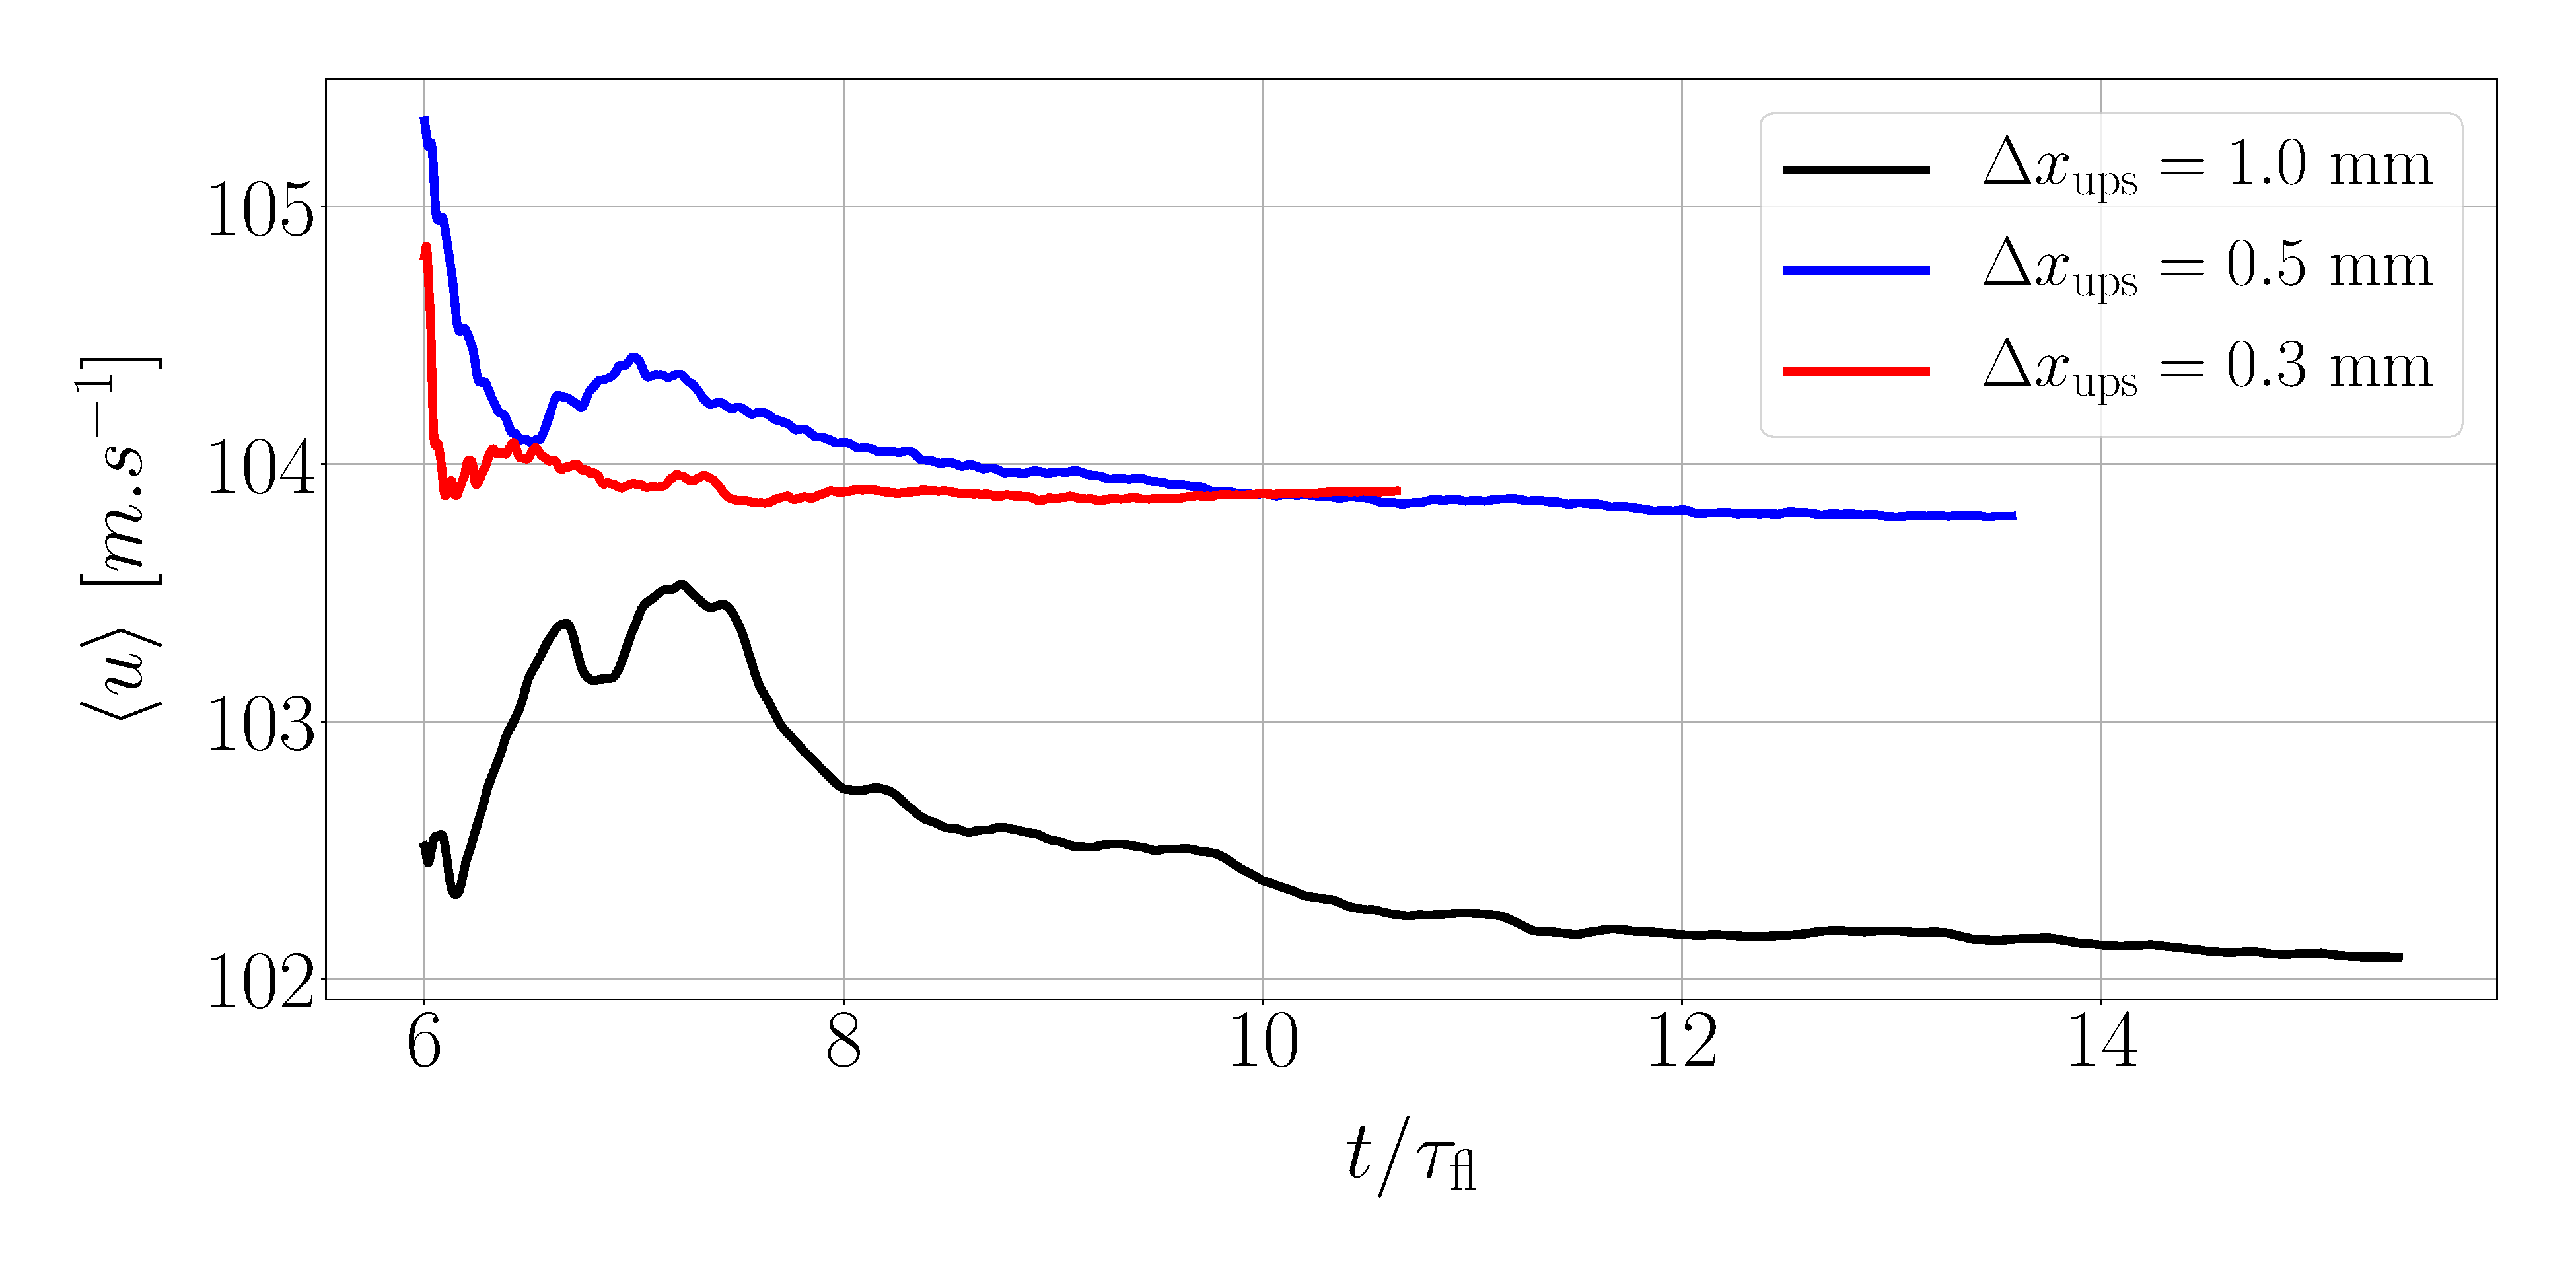
\includegraphics[scale=0.125]{./part2_developments/figures_ch5_resolved_JICF/results_ics_mesh_convergence_line_averages/U_MEAN.pdf}
   \vspace*{-0.30in}
   \caption{Mean axial velocity}
   %\label{} 
\end{subfigure}
\hfill
\begin{subfigure}[b]{0.45\textwidth}
	\centering
   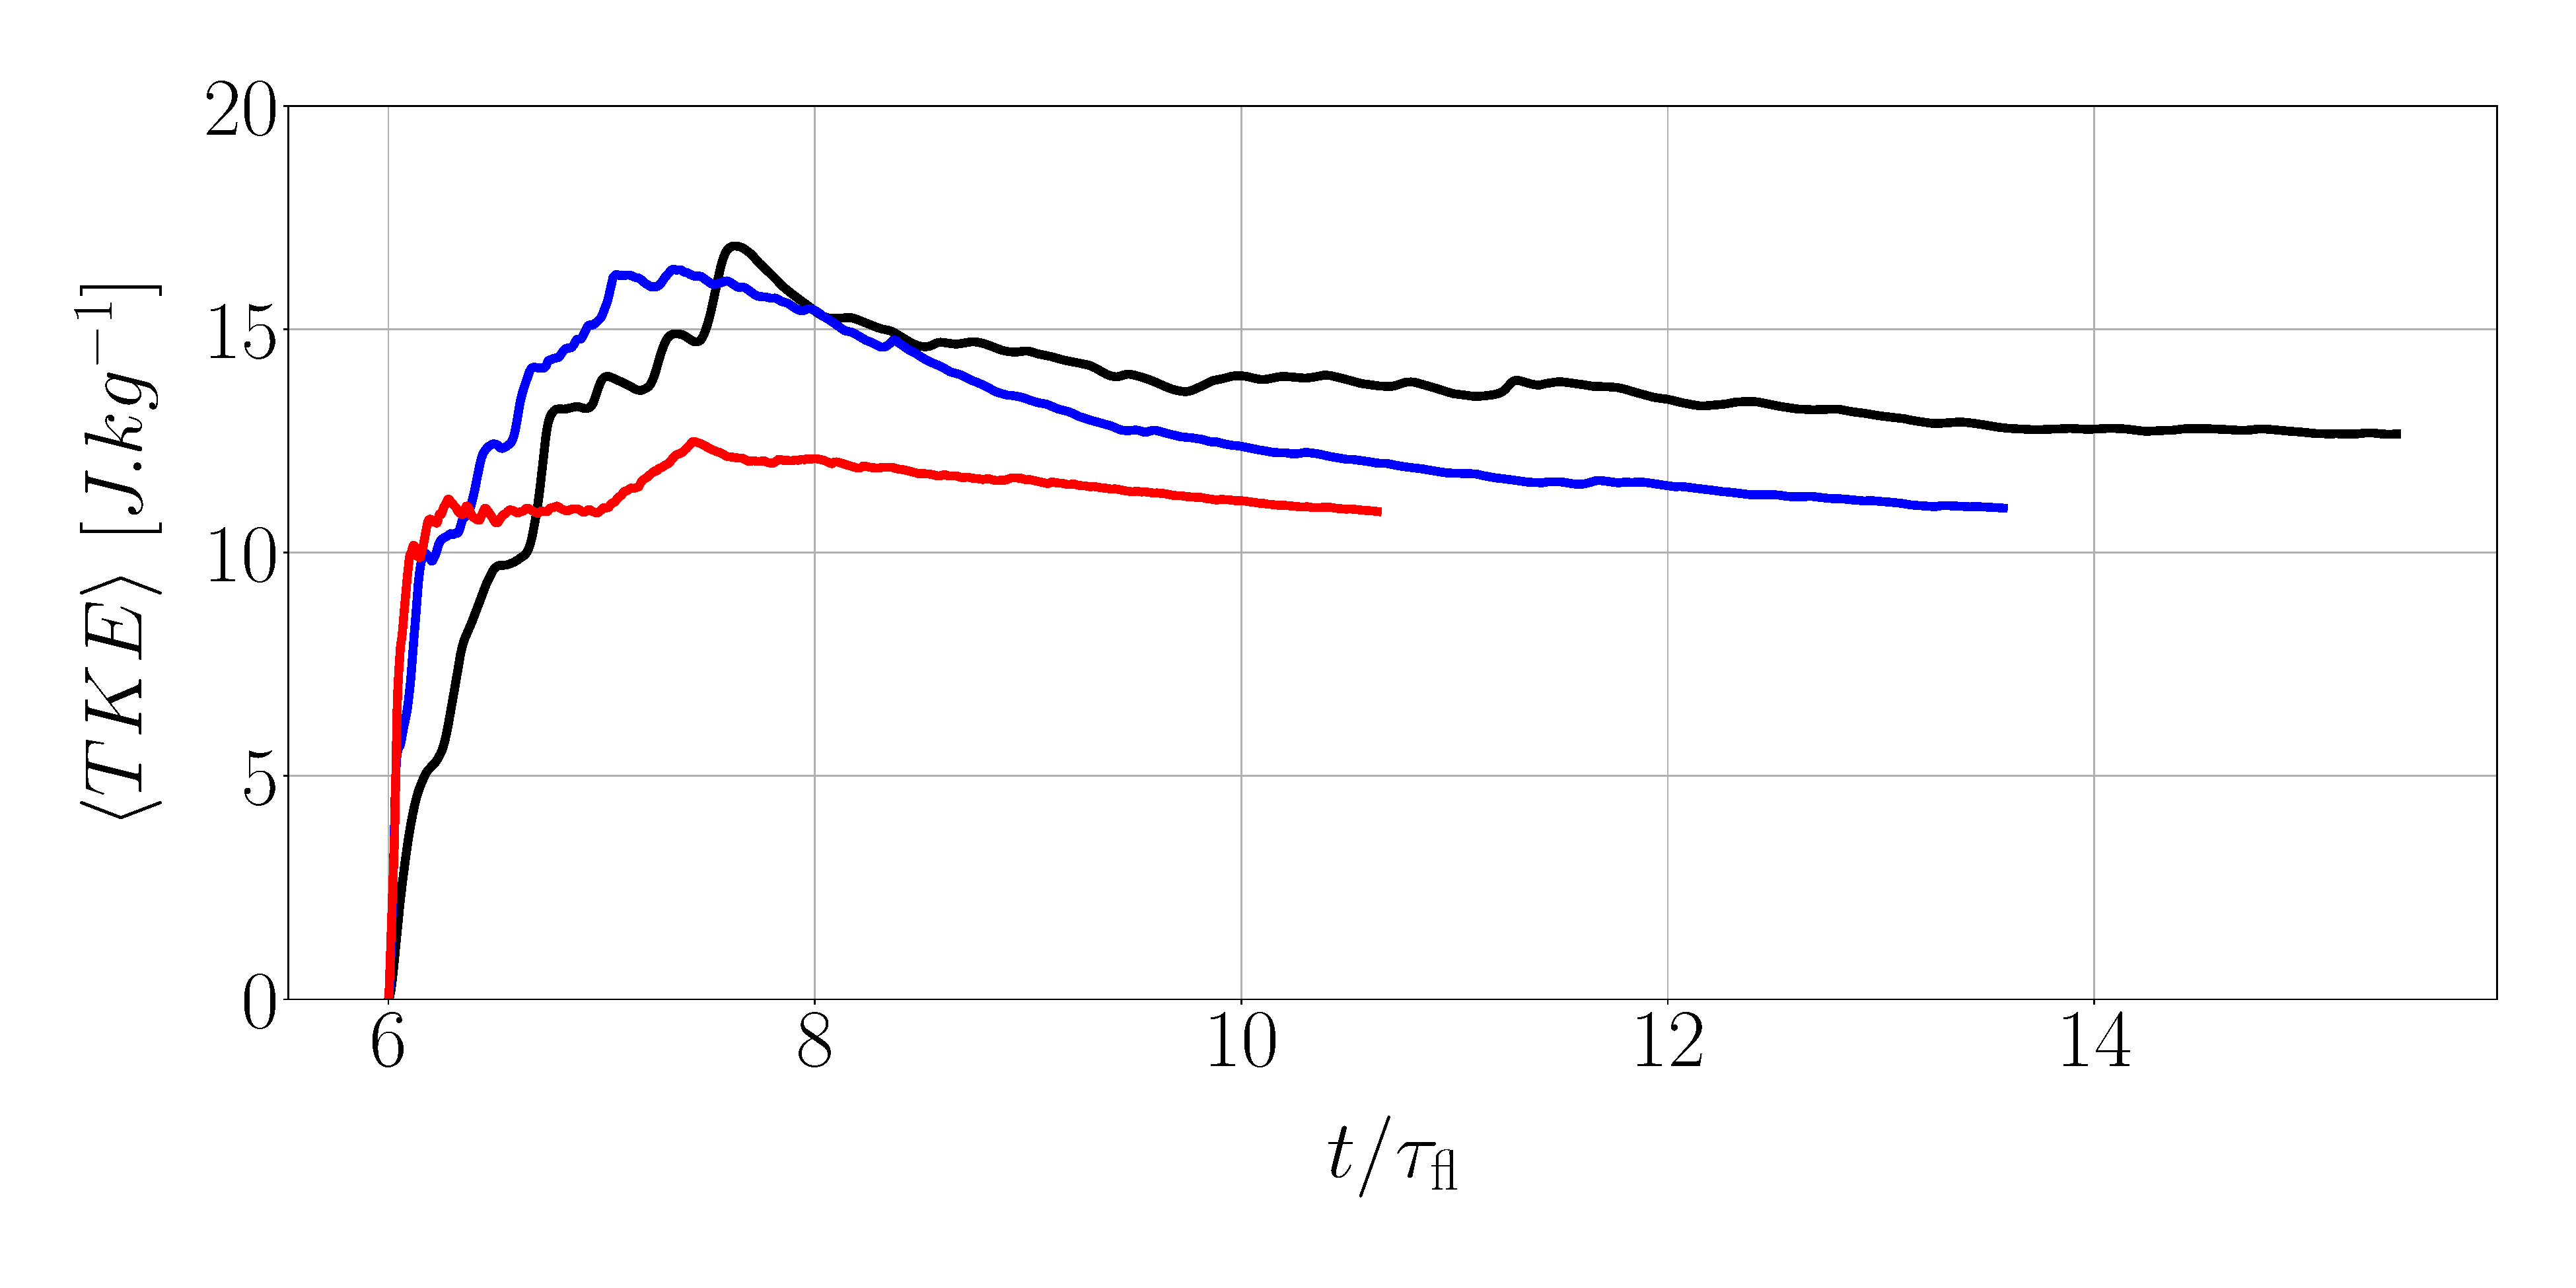
\includegraphics[scale=0.125]{./part2_developments/figures_ch5_resolved_JICF/results_ics_mesh_convergence_line_averages/TKE.pdf}
   \vspace*{-0.30in}
   \caption{Turbulent Kinetic Energy}
   %\label{}
\end{subfigure}
\caption{Convergence of line-integrated mean axial velocity and TKE with mesh resolution}
\label{fig:mesh_convergence_line_averages}
\end{figure}

\begin{figure}[ht]
\centering
\includeinkscape[inkscapelatex=false,scale=0.75]{./part2_developments/figures_ch5_resolved_JICF/results_ics_mesh_convergence_mesh_and_up/up_field_instantaneous_both}
\caption[Instantaneous $u'$ fields from gaseous simulation for the high Weber case]{Instantaneous $u'$ fields from gaseous simulation for the high Weber case. The right column shows a zoomed-in view of the dashed rectangle from the left column. Black contours indicate the lines with zero instantaneous fluctuation $u' = 0$. From top to bottom $\Delta x_\mathrm{ups} = 1, 0.5, 0.3$ mm.}
\label{fig:ics_mesh_independency_study_up_fields}
\end{figure}



Instantaneous snapshots of the fluctuating axial component $u'$ in the middle plane are shown in Figure \ref{fig:ics_mesh_independency_study_up_fields}. Adding turbulence at the inlet introduces fluctuations that are transported downstream the domain. When no turbulence is added, fluctuations are not present (the black contours at the inlet are due to small numerical fluctuations of $u'$) except close to the walls, since they are created inside the boundary layer where flow is intrinsically turbulent. It is also observed that the characteristic length of the eddies changes when refining the mesh: for the coarsest mesh ($\Delta x_\mathrm{ups} = 1$ mm), these structures are generally large, while refining the mesh to $\Delta x_\mathrm{ups} = 0.5$ and $0.3$ mm reduced their size. 


In order to compare quantitatively the difference between meshes, the signals of $u'$ have been monitored with time at the probes shown by the white crosses in the top of Figure \ref{fig:ics_mesh_independency_study_up_fields}. Two probes are located: one at 50 mm upstream the liquid inlet (x = 70 mm, probe A) and another one 1 mm upstream the liquid injection nozzle (x = 119 mm, probe B), both at a height of 8 mm from the bottom wall. The capability of the meshes to transport the resolved turbulent scales is then verified by comparing the fluctuations and spectra obtained with Fast Fourier Transform (FFT) at both probes in Figure \ref{fig:ics_mesh_independency_study_probes}. Time has been normalised with the flow-through time $\tau_\mathrm{fl}$, and the signals are shown for one passage of $\tau_\mathrm{fl}$ for easiness of visualization. For the coarsest mesh $\Delta x_\mathrm{ups} = 1$ mm (Figure \ref{fig:ics_mesh_independency_study_probes_dx1p0}), the $u'$ signal sampled closer to the nozzle (Probe B) shows similar magnitudes and frequencies to the signal sampled upstream (Probe A). Despite the characteristic peaks at frequencies of 8, 17 and 25 $\mathrm{kHz}$ with decreasing intensity for both probes, low frequencies below 10 $\mathrm{kHz}$ are excited. The spectrum at Probe B shows a higher relative intensity at these low frequencies with a peak at 3 $\mathrm{kHz}$ not observed at probe A. This indicates that for this resolution, turbulent energy is not properly transported to the liquid injector. Furthermore, characteristic frequencies larger than 25 $\mathrm{kHz}$ cannot be captured, which is not the case for the rest of resolutions. When the mesh is refined to $\Delta x_\mathrm{ups} = 0.5$ mm (Figure \ref{fig:ics_mesh_independency_study_probes_dx0p5}), the small dominant frequencies are no longer relevant and dominant frequencies are properly captured, as the match in the peaks of the spectra indicates. In this case, the frequencies 8 and 25 $\mathrm{kHz}$ have larger intensity than 17 $\mathrm{kHz}$. Refining the mesh to $\Delta x_\mathrm{ups} = 0.3$ mm (Figure \ref{fig:ics_mesh_independency_study_probes_dx0p3}) has no longer effect neither in the magnitude of the fluctuations nor in the spectrum. 

The fluctuations and FFT of the simulation performed without turbulence injection for the resolution $\Delta x_\mathrm{ups} = 0.5$ mm are shown Figure \ref{fig:ics_mesh_independency_study_probes_dx0p5_no_turb}. As expected, the magnitude of the fluctuations is lower than in the cases with synthetic turbulence. The spectrum shows that the energy content at low frequencies is high and that no clear dominant frequencies are found. \\



A final verification on the mesh capability to transport turbulent energy is done by calculating the Turbulent Kinetic Energy (TKE) at the probes A and B for simulation where turbulence is transported. TKE is defined as follows:

\begin{equation}
\label{eq:TKE_general_defintion}
TKE = \frac{1}{2} \left( \overline{u'^2} + \overline{v'^2} + \overline{w'^2} \right)
\end{equation}

\clearpage

\begin{figure}[ht]
\centering
\begin{subfigure}[b]{1.0\textwidth}
	\centering   
	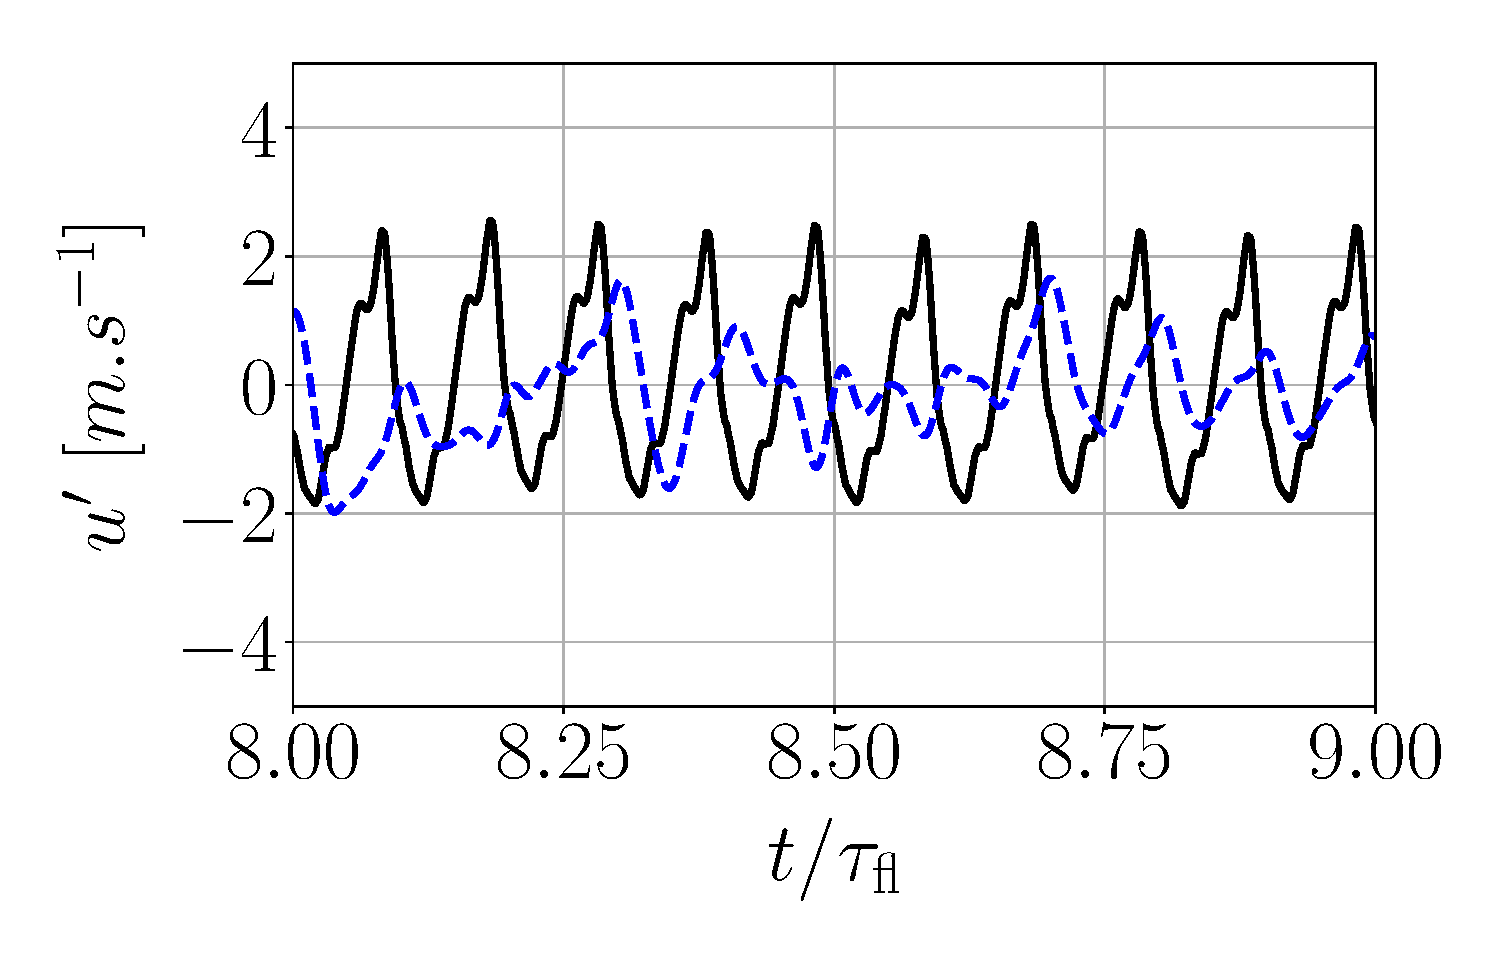
\includegraphics[scale=0.28]{./part2_developments/figures_ch5_resolved_JICF/results_ics_mesh_convergence_probes/up_dx1p0.pdf}
	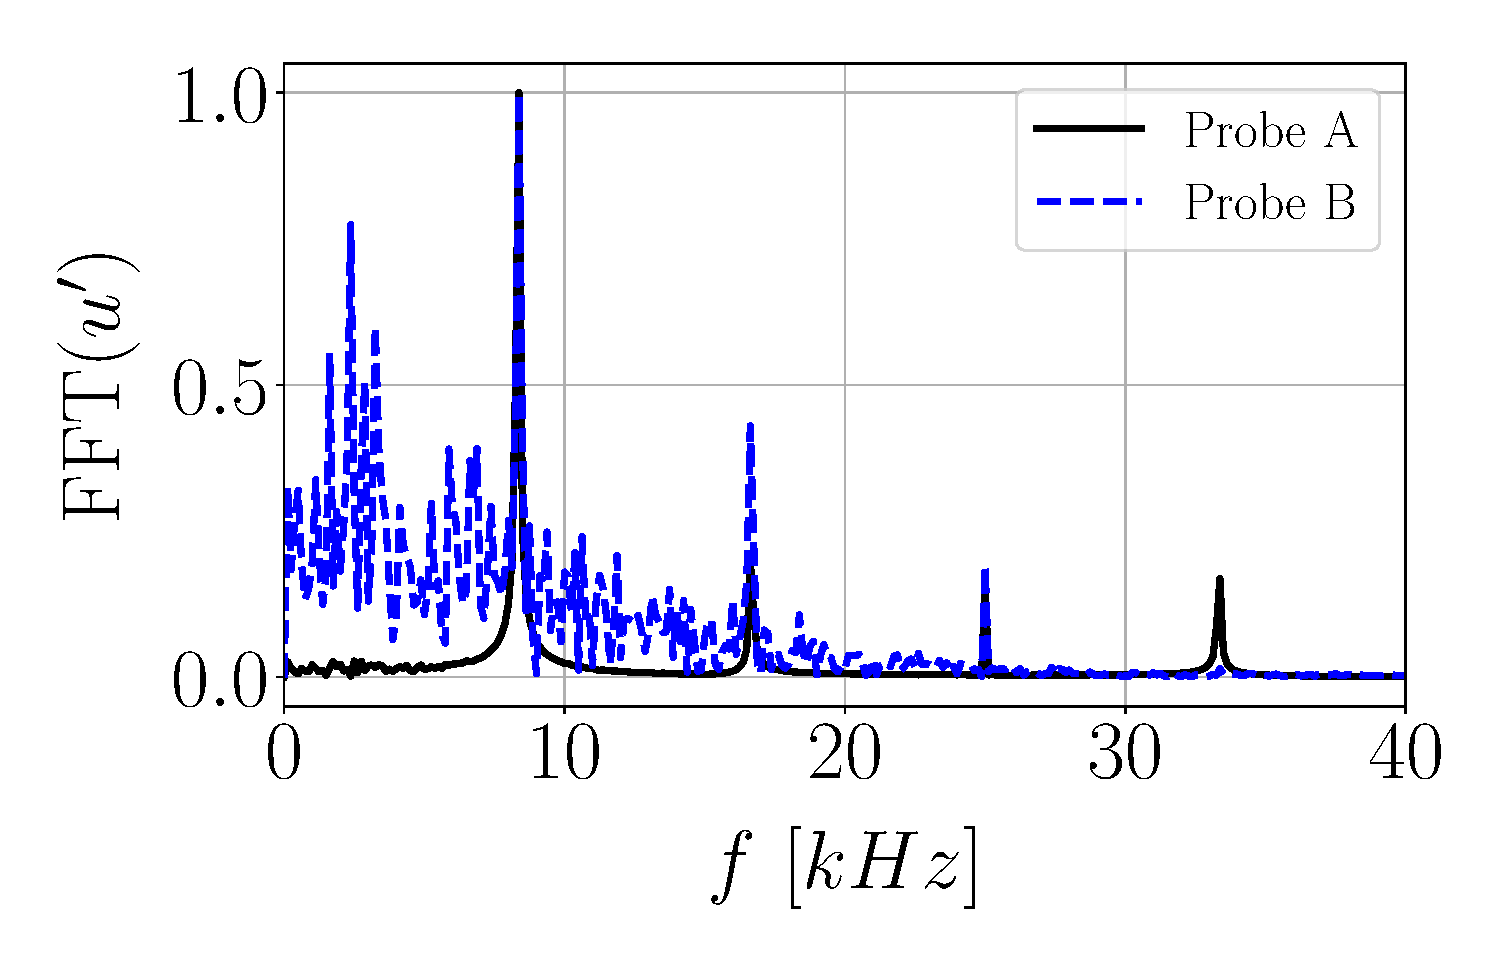
\includegraphics[scale=0.28]{./part2_developments/figures_ch5_resolved_JICF/results_ics_mesh_convergence_probes/spectra_linear_scale_dx1p0.pdf}
%	\subfloat[\centering]{{\includegraphics[scale=0.20]{./part2_developments/figures_ch5_resolved_JICF/results_ics_mesh_convergence_probes/up_dx1p0.eps} }}%
%    \qquad
%    \subfloat[\centering]{{ \includegraphics[scale=0.20]{./part2_developments/figures_ch5_resolved_JICF/results_ics_mesh_convergence_probes/spectra_linear_scale_dx1p0.eps} }}%
   \vspace*{-0.10in}
   \caption{Mesh $\Delta x_\mathrm{ups} = 1$ mm}
   \label{fig:ics_mesh_independency_study_probes_dx1p0}
\end{subfigure}


\vskip\baselineskip

\begin{subfigure}[b]{1.0\textwidth}
	\centering
   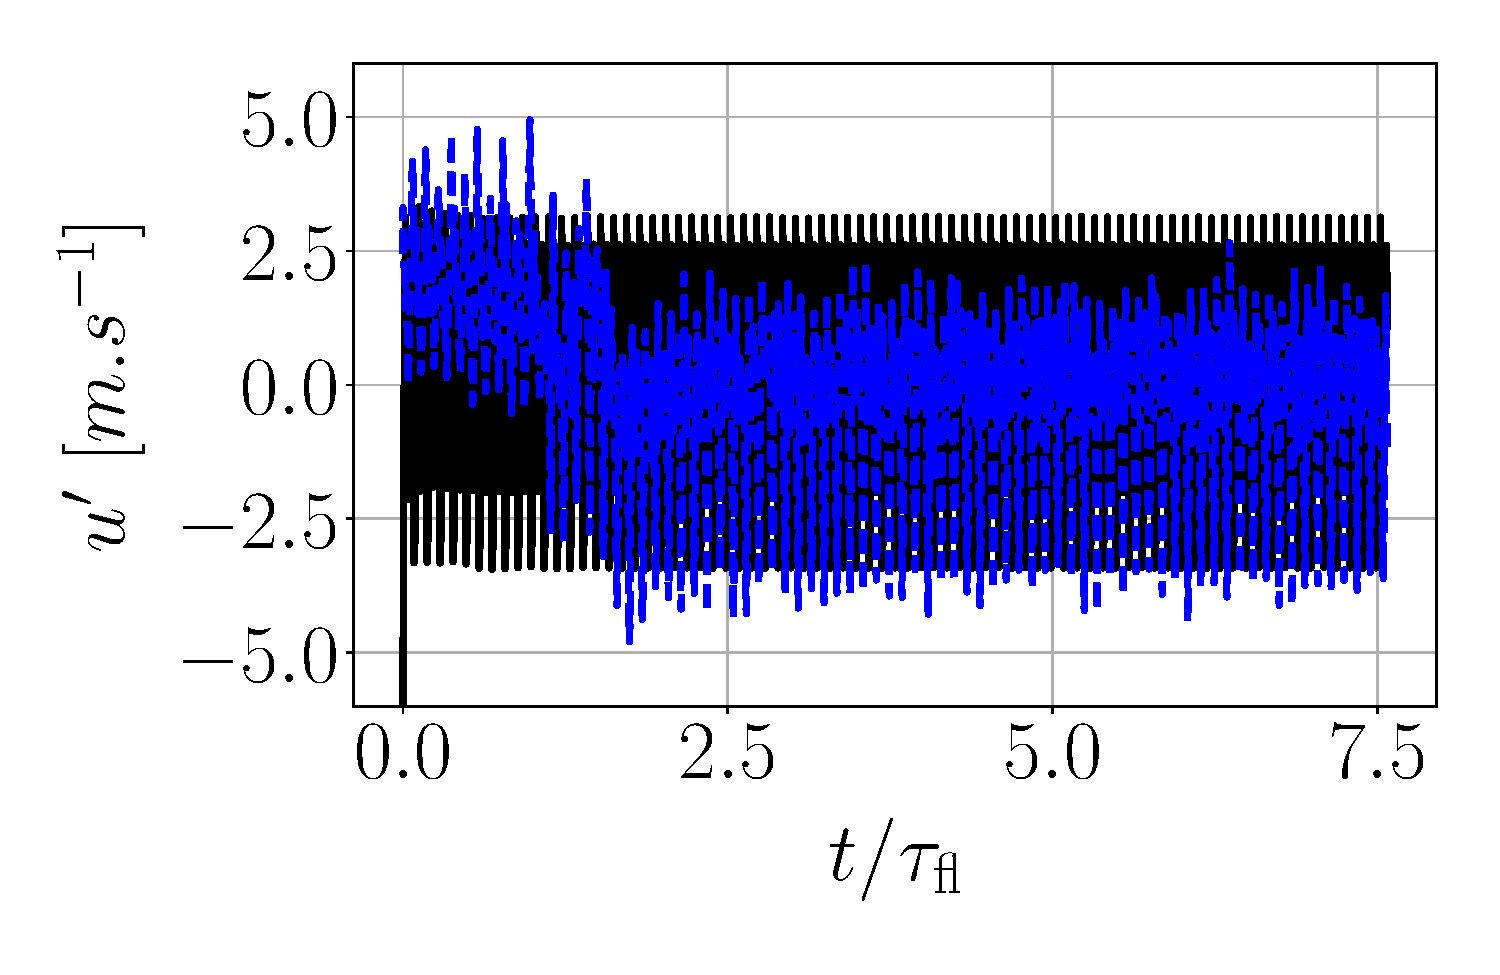
\includegraphics[scale=0.28]{./part2_developments/figures_ch5_resolved_JICF/results_ics_mesh_convergence_probes/up_dx0p5.pdf}
   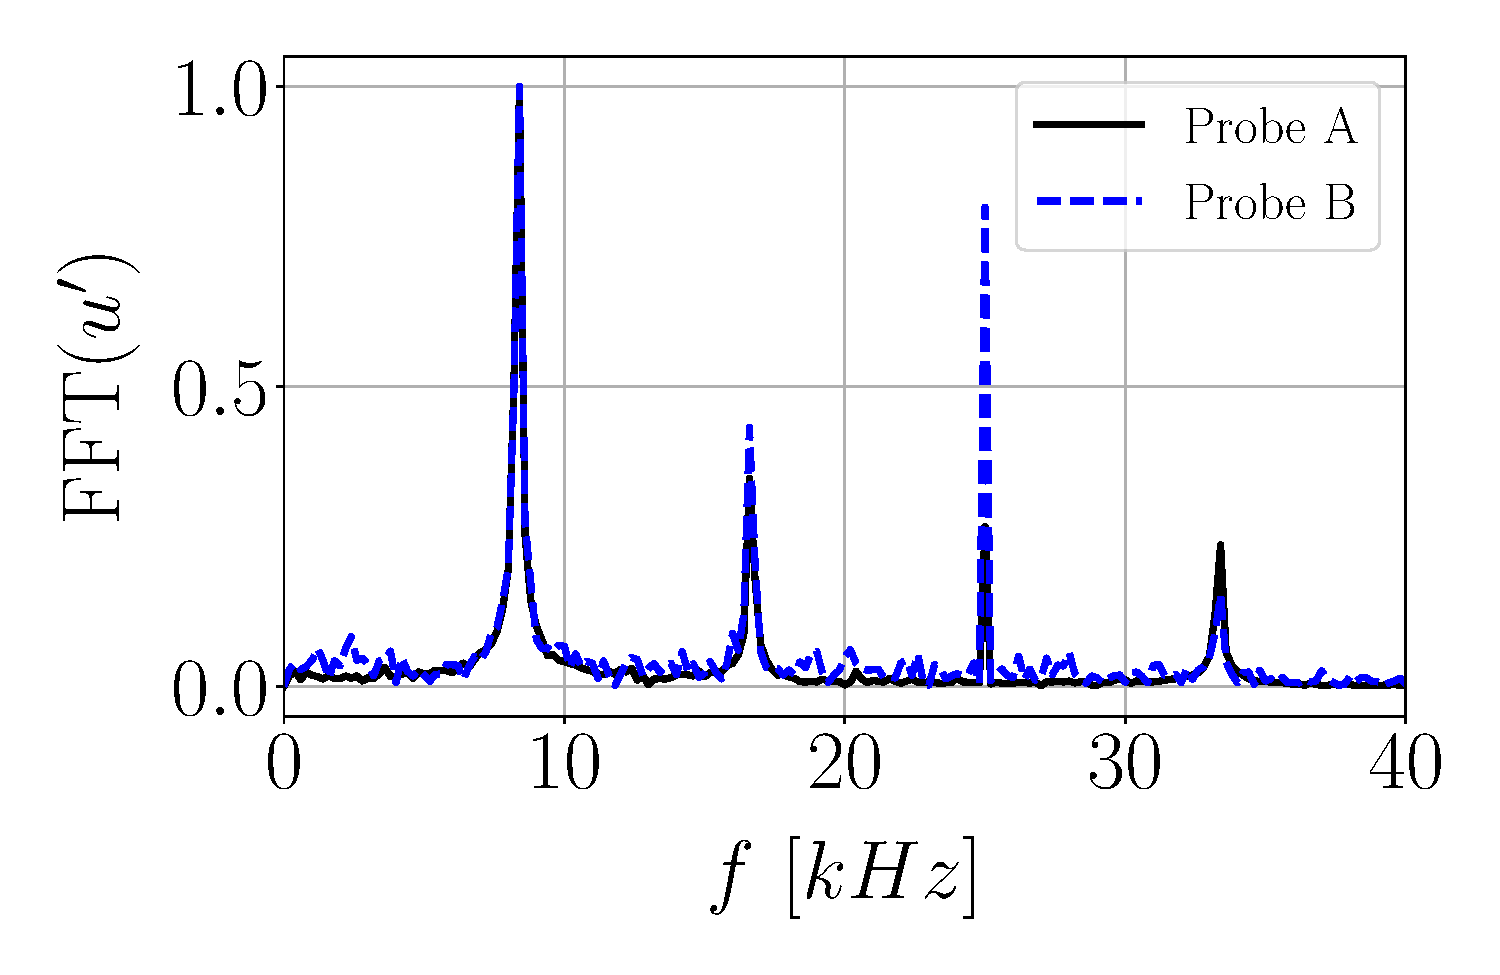
\includegraphics[scale=0.28]{./part2_developments/figures_ch5_resolved_JICF/results_ics_mesh_convergence_probes/spectra_linear_scale_dx0p5.pdf}
   \vspace*{-0.10in}
   \caption{Mesh $\Delta x_\mathrm{ups} = 0.5$ mm}
   \label{fig:ics_mesh_independency_study_probes_dx0p5}
\end{subfigure}

\vskip\baselineskip

\begin{subfigure}[b]{1.0\textwidth}
	\centering
   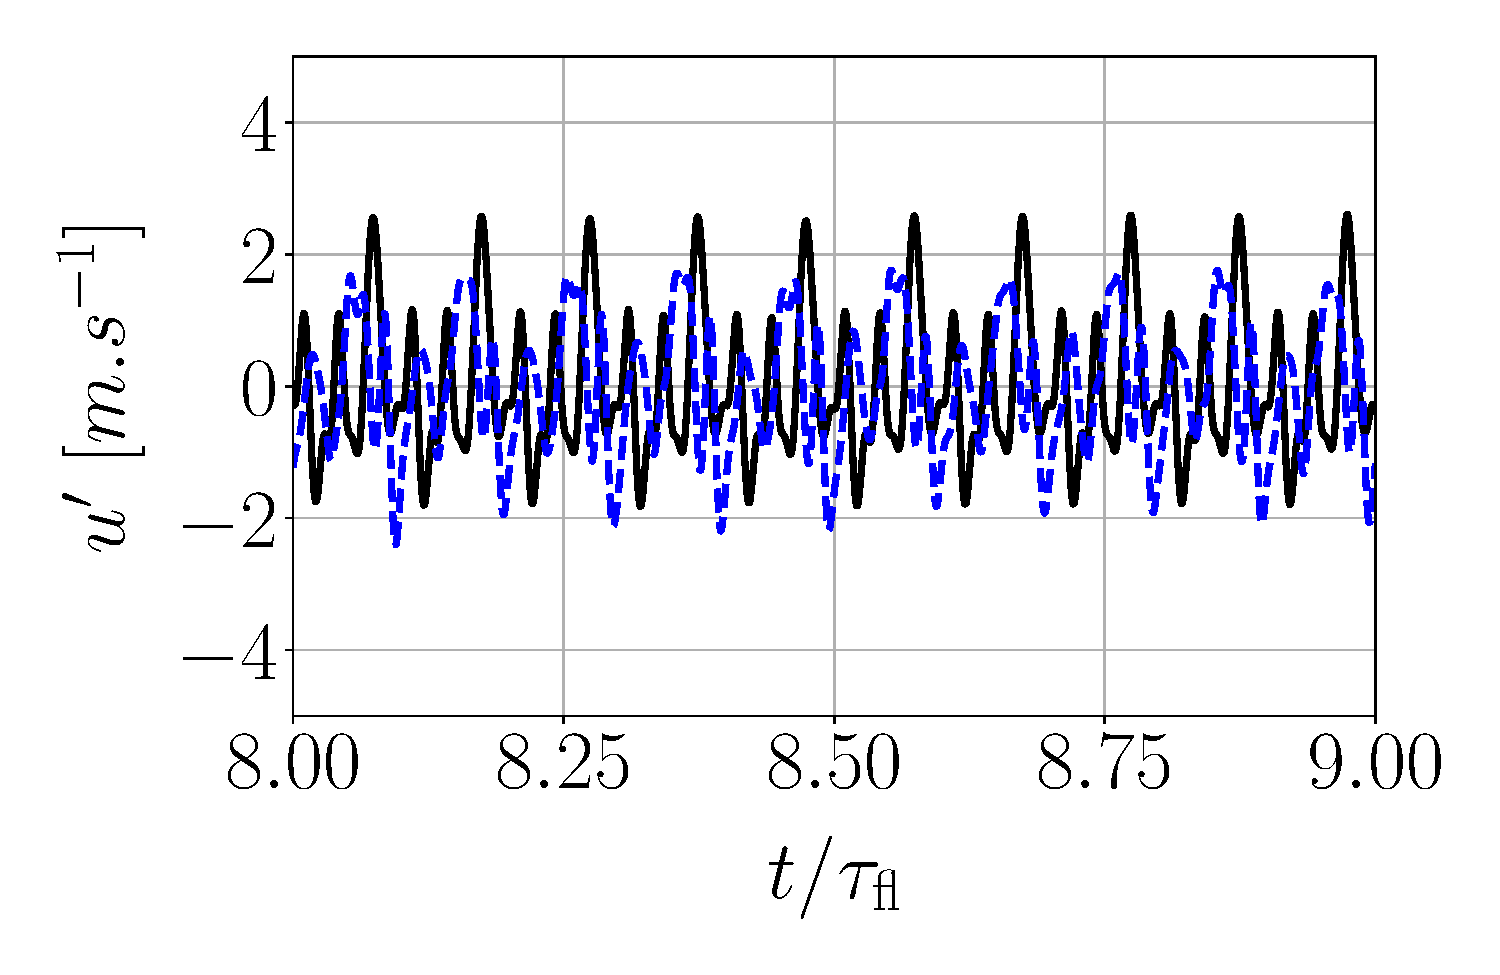
\includegraphics[scale=0.28]{./part2_developments/figures_ch5_resolved_JICF/results_ics_mesh_convergence_probes/up_dx0p3.pdf}
   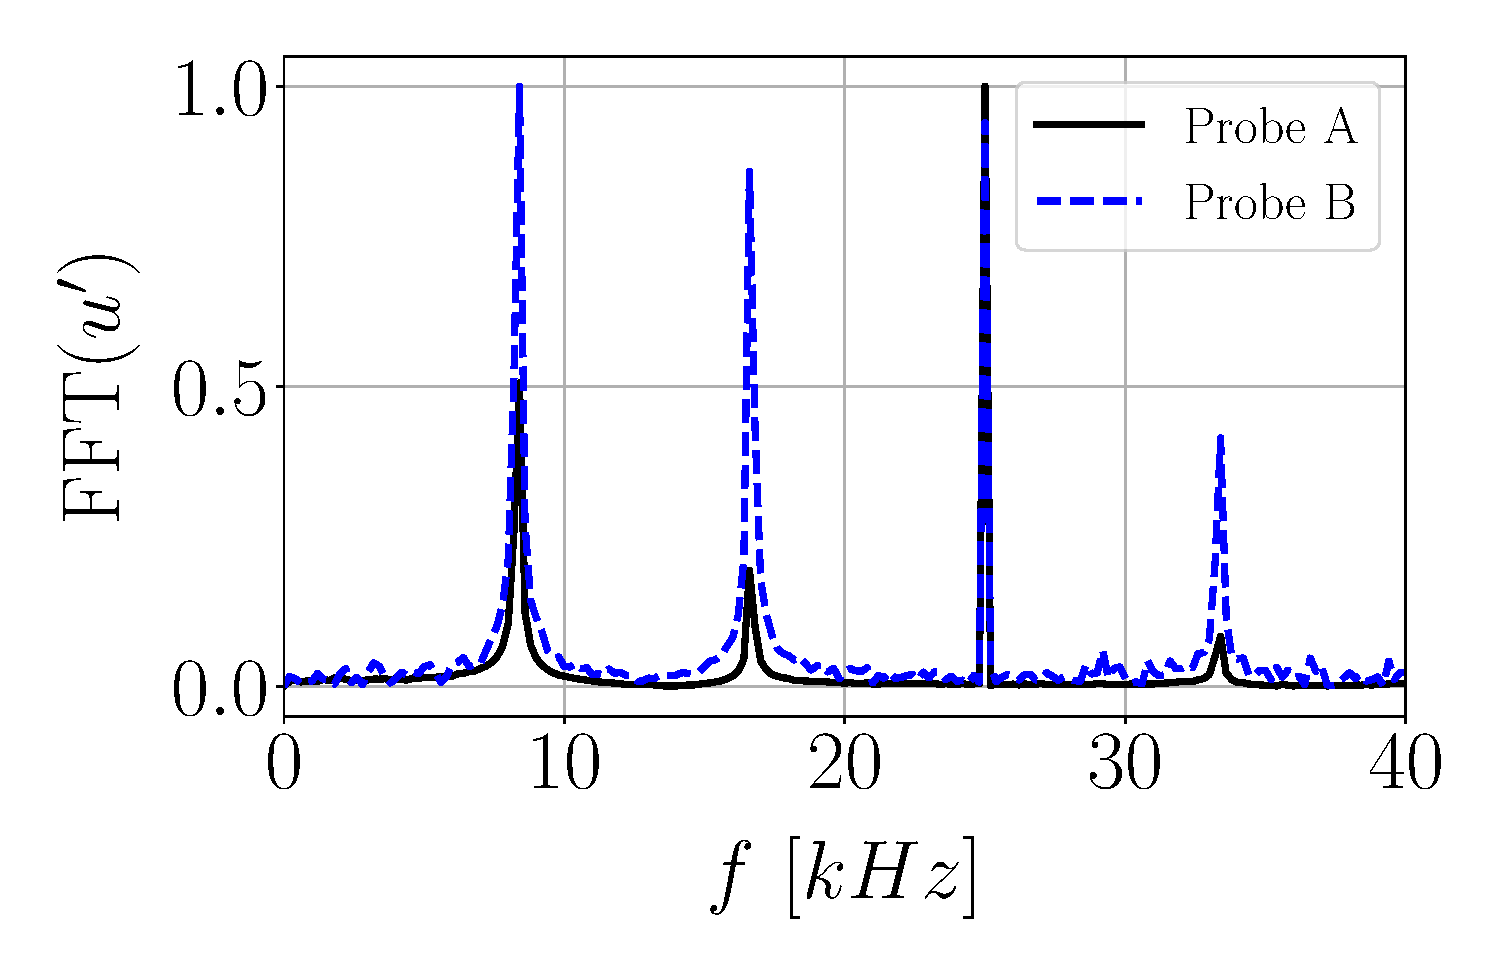
\includegraphics[scale=0.28]{./part2_developments/figures_ch5_resolved_JICF/results_ics_mesh_convergence_probes/spectra_linear_scale_dx0p3.pdf}
   \vspace*{-0.10in}
   \caption{{Mesh $\Delta x_\mathrm{ups} = 0.3$ mm}}
   \label{fig:ics_mesh_independency_study_probes_dx0p3}
\end{subfigure}


\vskip\baselineskip

\begin{subfigure}[b]{1.0\textwidth}
	\centering
   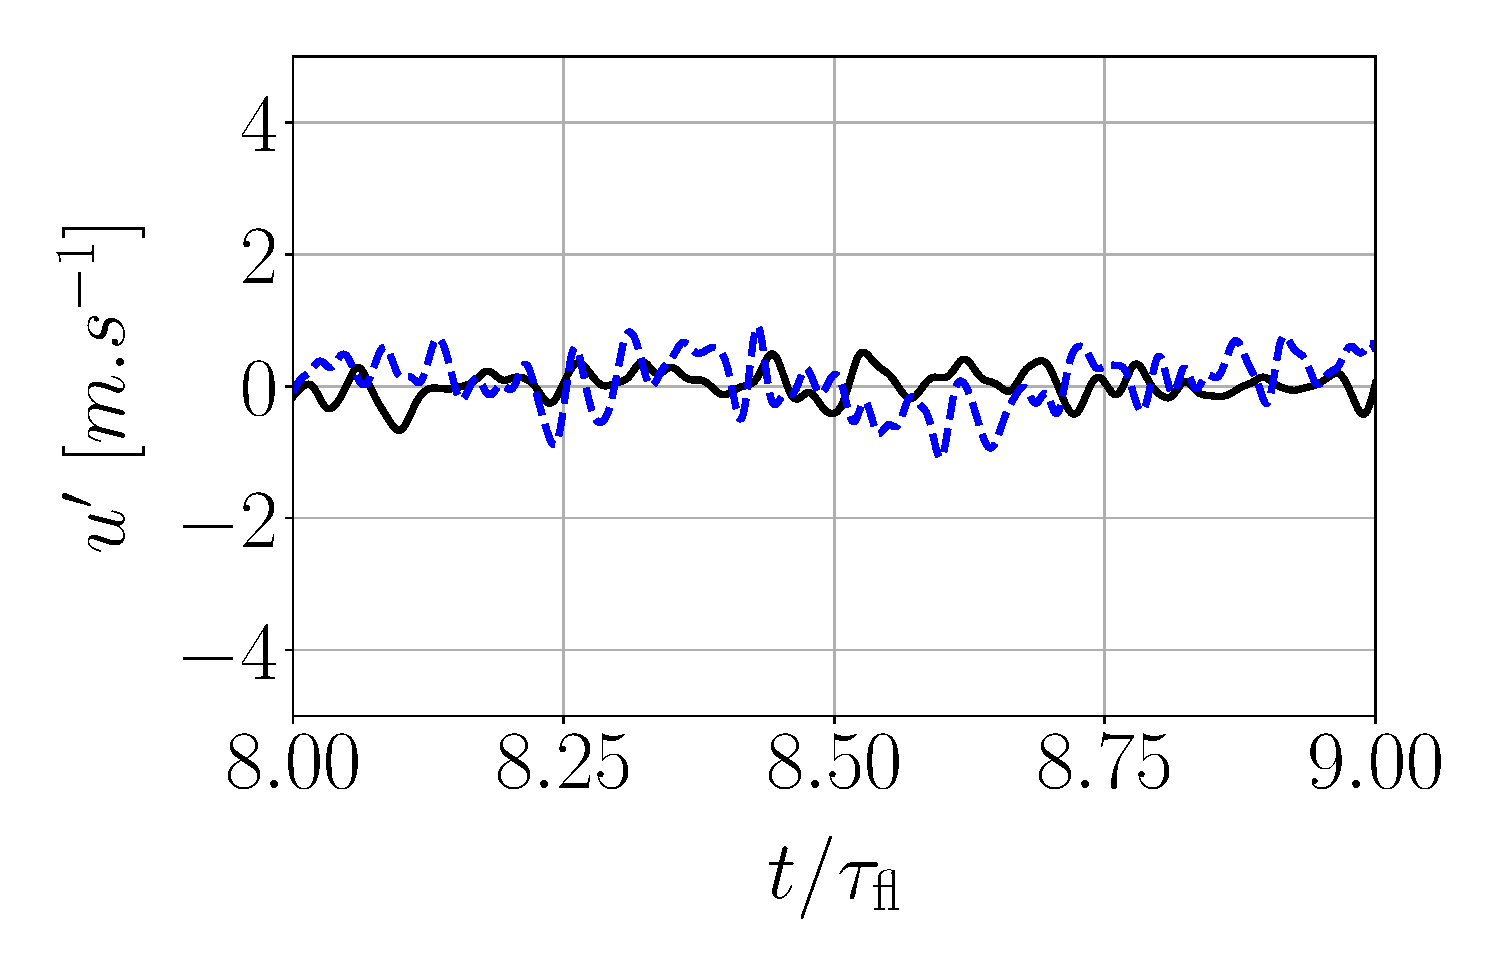
\includegraphics[scale=0.28]{./part2_developments/figures_ch5_resolved_JICF/results_ics_mesh_convergence_probes/up_dx0p5_no_turb.pdf}
   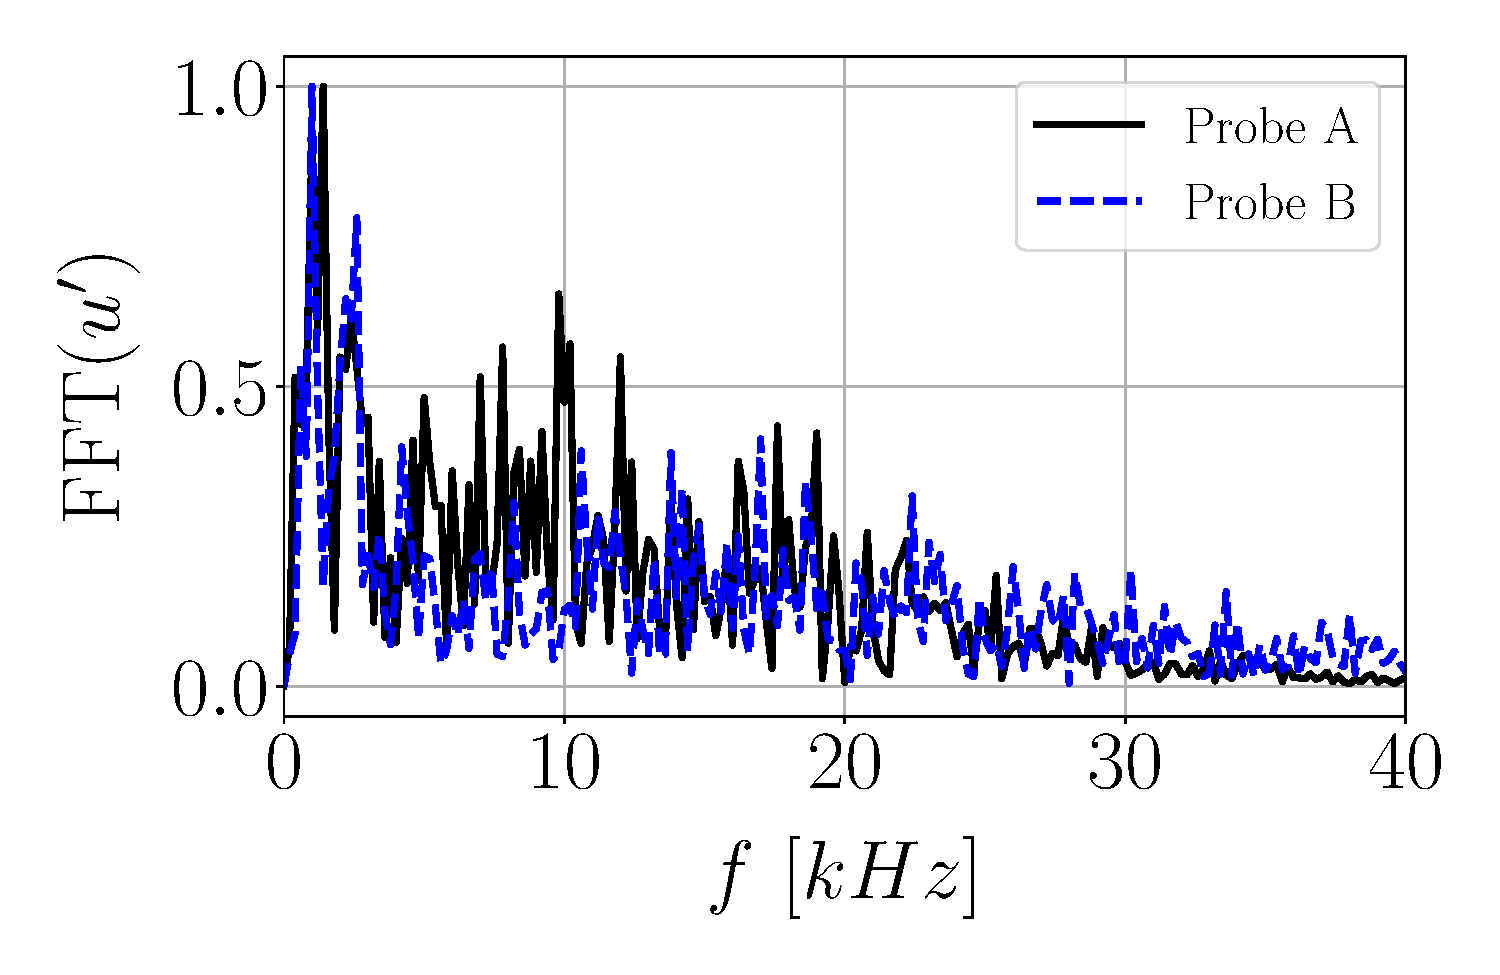
\includegraphics[scale=0.28]{./part2_developments/figures_ch5_resolved_JICF/results_ics_mesh_convergence_probes/spectra_linear_scale_dx0p5_no_turb.pdf}
   \vspace*{-0.10in}
   \caption{Mesh $\Delta x_\mathrm{ups} = 0.5$ mm without turbulence injection}
   \label{fig:ics_mesh_independency_study_probes_dx0p5_no_turb}
\end{subfigure}

\caption[Axial velocity fluctuations and associated frequencies at the sampling probes for the simulations at high Weber number.]{
Axial velocity fluctuations and associated frequencies at the sampling probes for the simulations at high Weber number. \textsl{Left}: $u'$ fluctuations. \textsl{Right}: spectra of the fluctuations obtained through FFT.}
\label{fig:ics_mesh_independency_study_probes}
\end{figure}


\clearpage



Note that, unlike in Eq. (\ref{eq:line_averaged_u_and_TKE}), the TKE is not line-averaged but represents the resolved energy contained in the eddies at the probes location. 
Figure \ref{fig:TKE_vs_dx_in_probes} gives the results. The coarser mesh with $\Delta x_\mathrm{ups} = 1$ mm provides different values of TKE in both probes with a difference of 34 $\%$: TKE is lost from point A to point B and this mesh cannot transport turbulence properly. Refining to $\Delta x_\mathrm{ups} = 0.5$ mm improves the transport capability of the mesh and both probes show similar values of TKE: 4.17 $J ~ kg^{-1}$ for probe A against 4.14 $J ~ kg^{-1}$ at probe B, making a difference of 0.7 $\%$. Finally, the mesh with $\Delta x_\mathrm{ups} = 0.3$ mm provides values of $4.2$ and $4.19$ $J ~ kg^{-1}$ in probes A and B respectively, yielding a difference of 0.24 $\%$ and making this mesh more suitable for transporting the turbulence. Nevertheless, the mesh with $\Delta x_\mathrm{ups} = 0.5$ mm already yields small errors in the TKE transport while providing TKE values very close to those of the mesh with $\Delta x_\mathrm{ups} = 0.3$ mm: it provides also good turbulent transport capabilities with smaller computational cost than the finest mesh due to its smaller number of elements (see Table \ref{tab:jicf_mesh_independence_gaseous_study}). 

\vspace*{-0.05in}

\begin{figure}[ht]
	\centering
	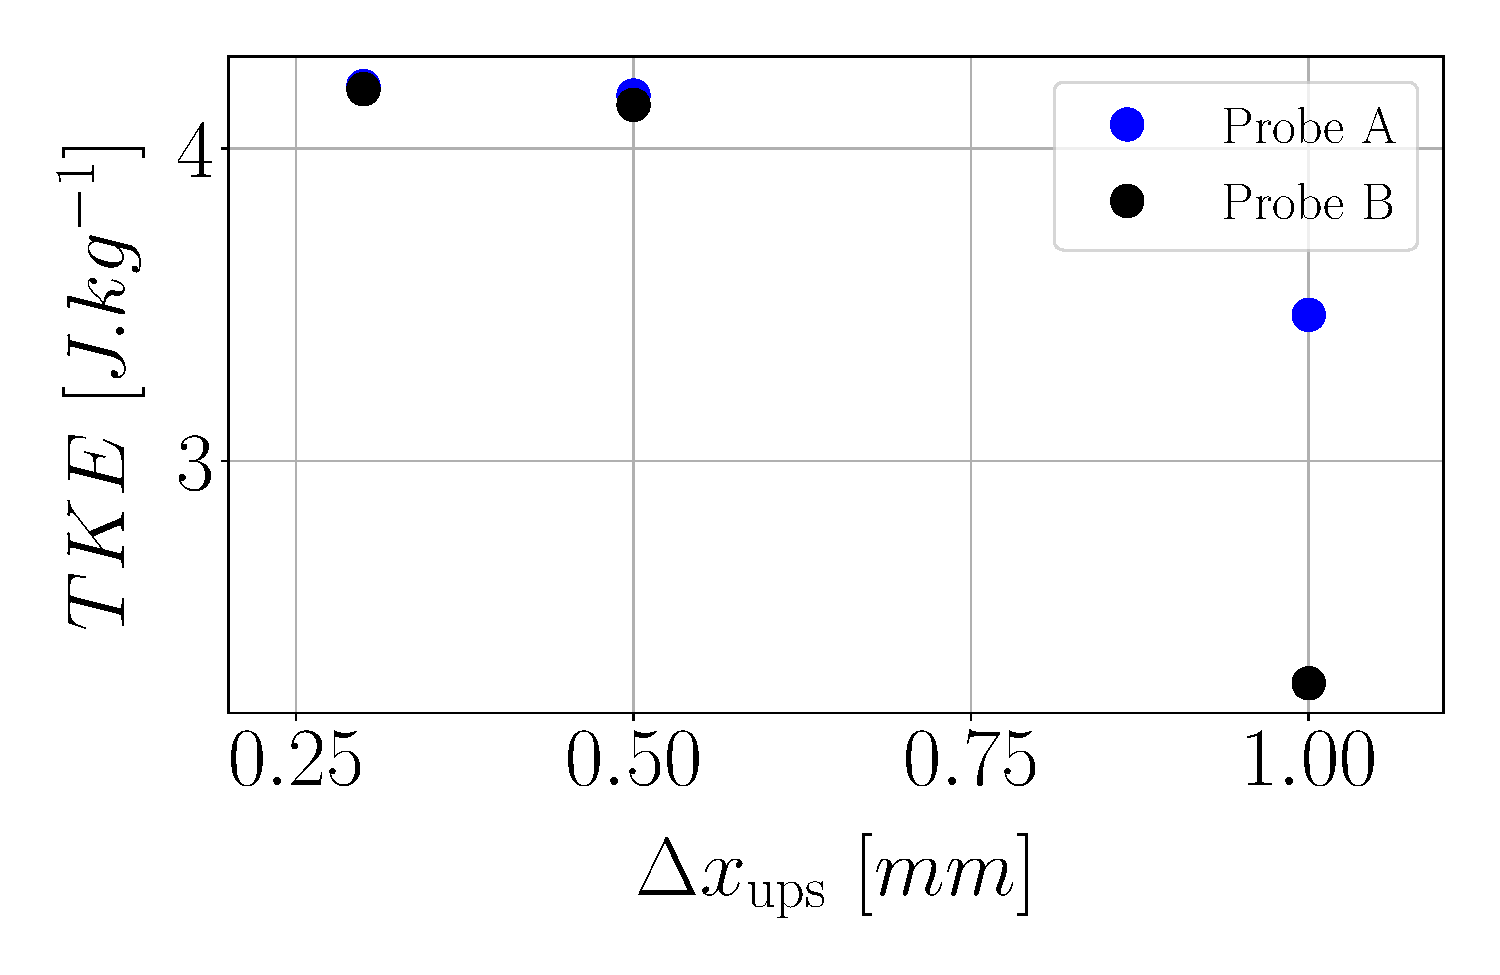
\includegraphics[scale=0.28]{./part2_developments/figures_ch5_resolved_JICF/results_ics_mesh_convergence_probes/TKE_vs_dx_in_probes.pdf}
   \vspace*{-0.15in}
   \caption{Variation in Turbulent Kinetic Energy in probes A and B with upstream mesh resolution.}
   \label{fig:TKE_vs_dx_in_probes}
\end{figure}

\vspace*{-0.05in}

Finally, Figure \ref{fig:ics_mesh_independency_study_mean_profiles} plots the profiles of mean axial velocity $\overline{u}$ and TKE along the vertical line from in Figure \ref{fig:ics_mesh_independency_study_up_fields} right. $\overline{u}$ is properly captured for all meshes, despite slight variations within the boundary layer where it evolves from 0 to the velocity in the outer layer, which is constant and equal in all cases (despite some fluctuations due to numerical noise). The boundary layer thickness (observed in the evolution of both $\overline{u}$ and $TKE$) is around 5 mm, which is consistent with the experimental values reported in \citeColor[becker_breakup_2002]. $TKE$ profiles in turbulent cases show that the turbulent energy in the outer layer (z > 5 $mm$) is similar for resolutions $\Delta x_\mathrm{ups} = 0.5$ and $0.3$ mm, but lower for the thicker resolution of 1 mm. Within the boundary layer, however, convergence with resolution is never achieved. Effectively, Kolmogorov length-scales for the studied case, which correspond to the length of the smallest eddies in the boundary layer, are of the order of $\eta \sim 0.5$ $\mu$m (see Table \ref{tab:jicf_characteristic_scales_kolmogovor} for estimations), which cannot be captured with any resolution employed. A proper resolution at this region would require a DNS study, which is nowadays unfeasible for the operating point studied and which justifies the use of LES for these simulations. Nevertheless, the values of TKE for z > 2 mm, including the energy decrease from this point up to the freestream, is converged for the resolution $\Delta x_\mathrm{ups} = 0.5$ mm. 


\begin{figure}[ht]
\centering
\begin{subfigure}[b]{0.45\textwidth}
	\centering
   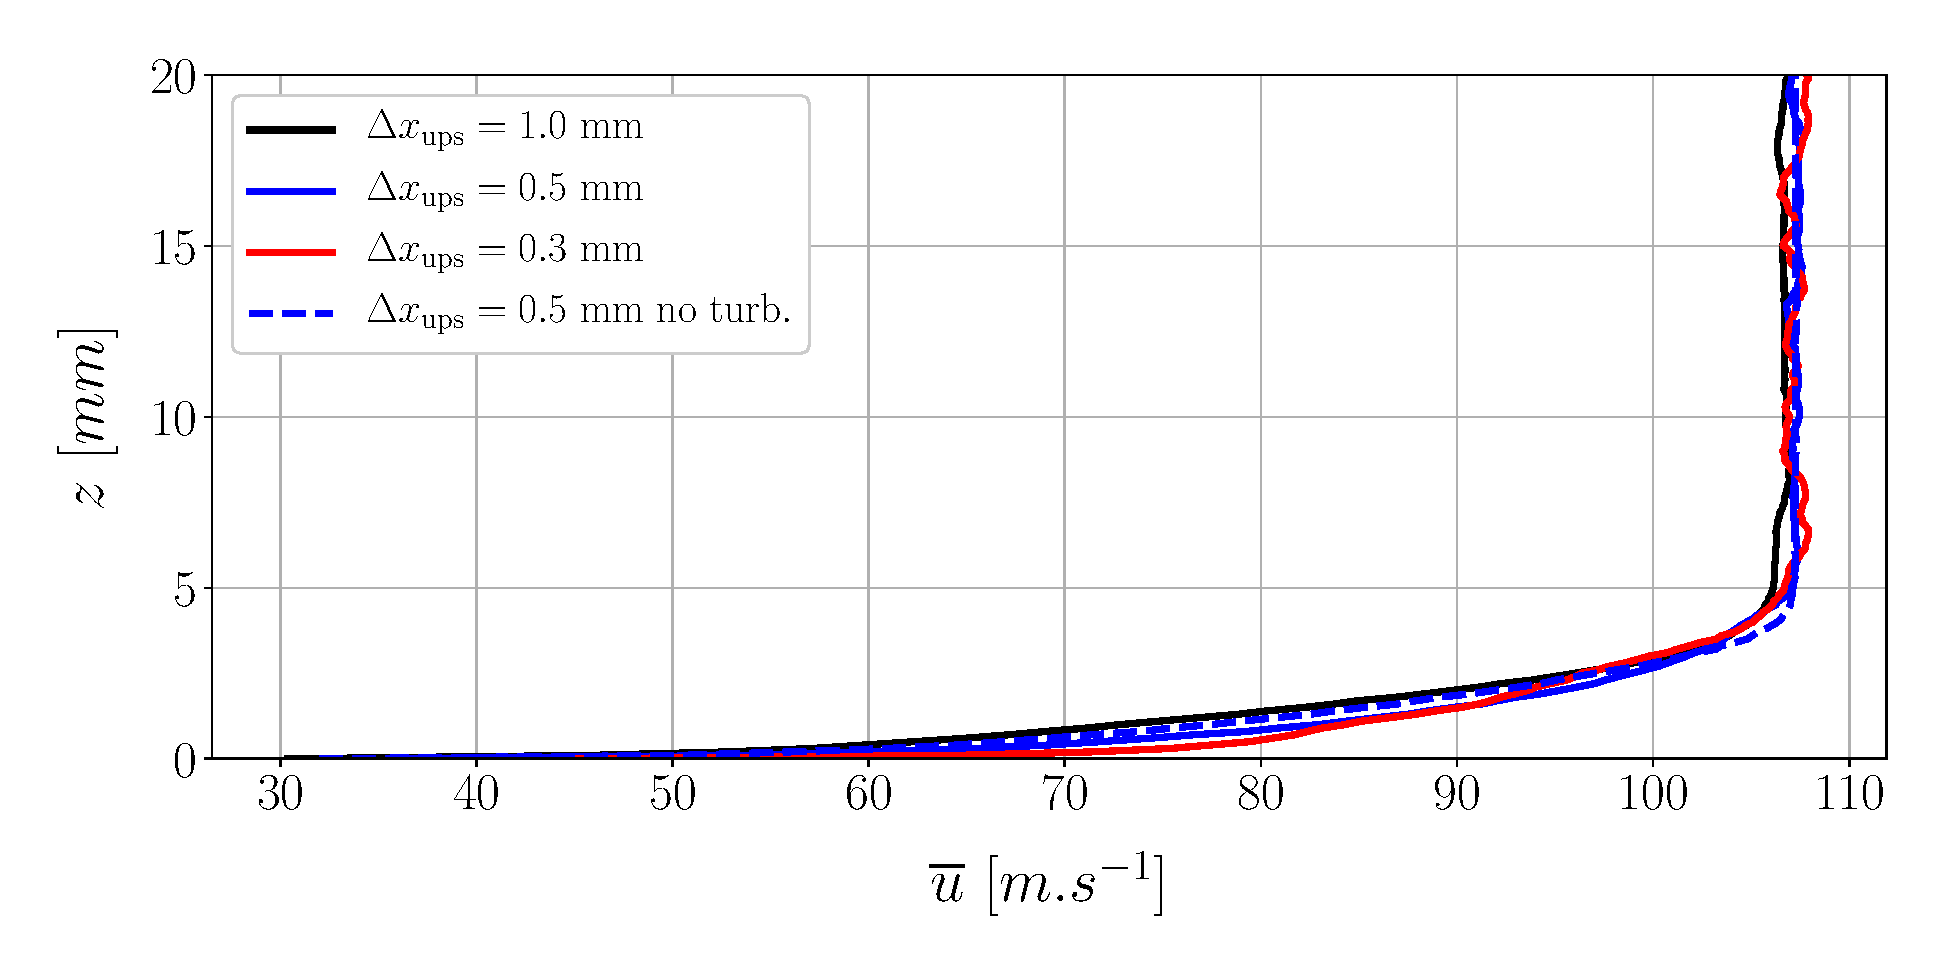
\includegraphics[scale=0.25]{./part2_developments/figures_ch5_resolved_JICF/results_ics_mesh_convergence_mean_profiles/U_MEAN_profiles.pdf}
   \vspace*{-0.20in}
   \caption{Mean axial velocity}
   %\label{} 
\end{subfigure}
\hfill
\begin{subfigure}[b]{0.45\textwidth}
	\centering
   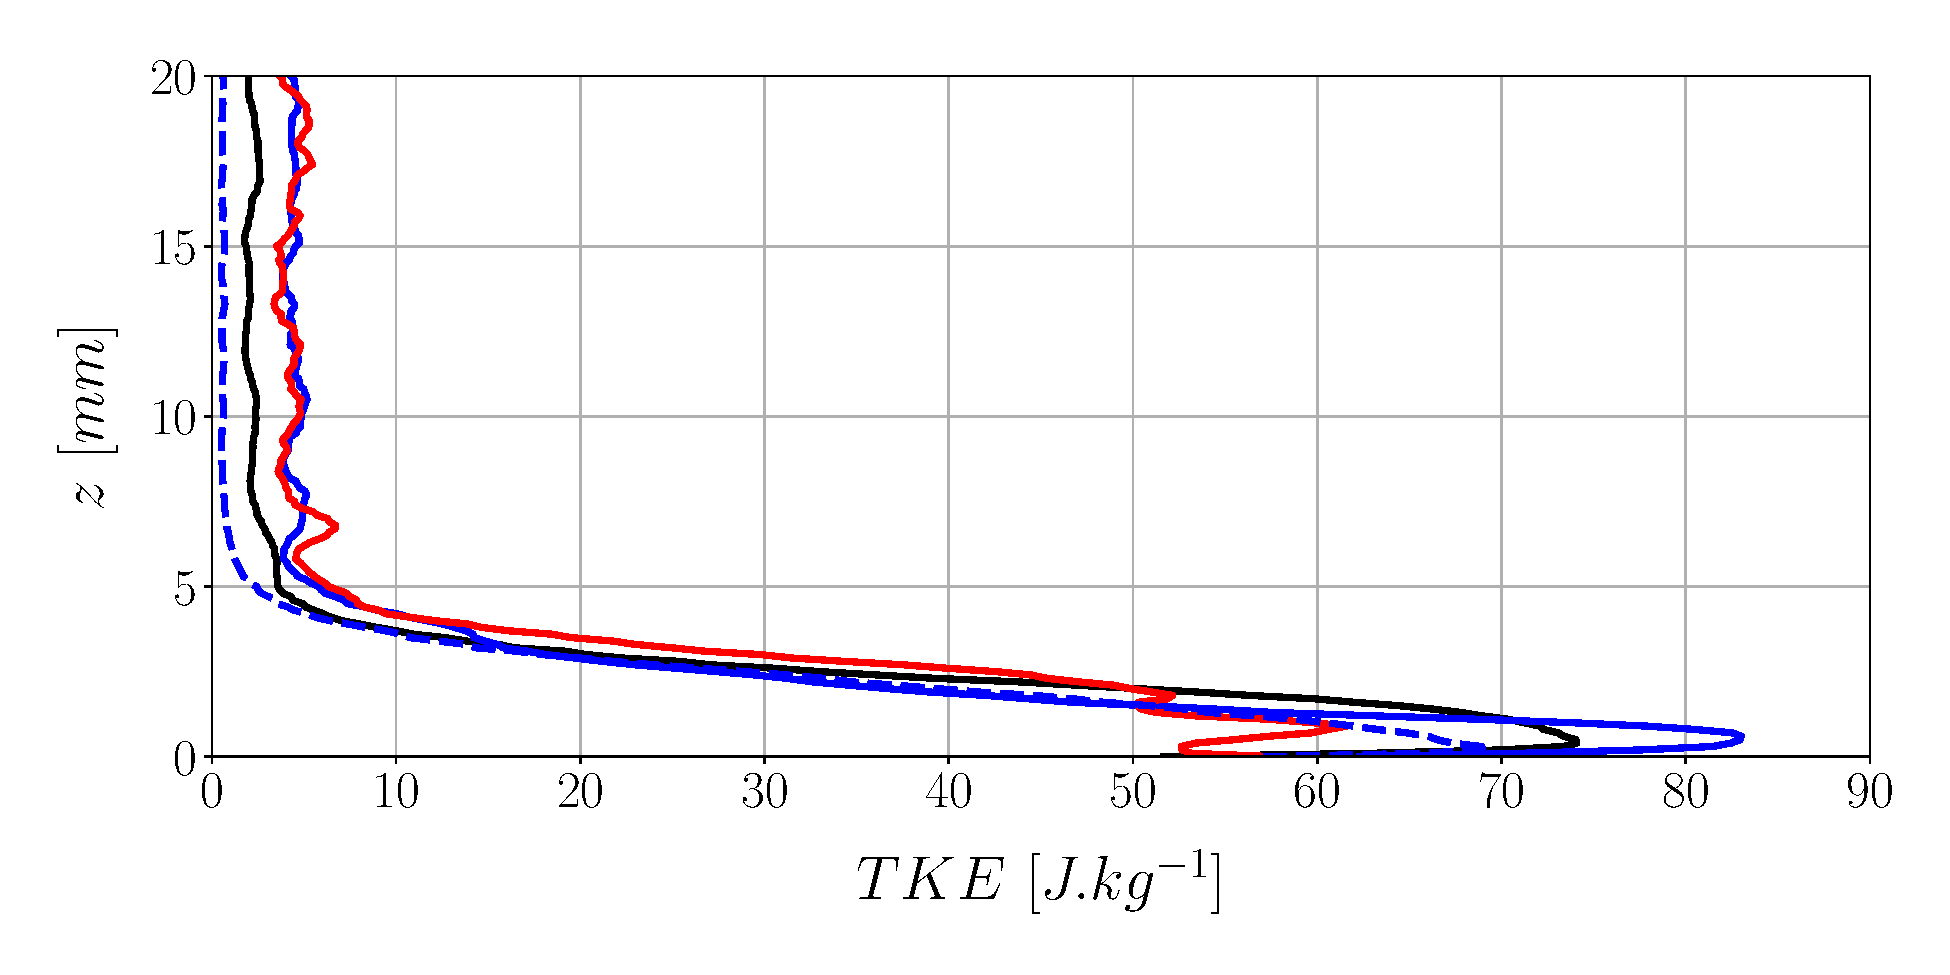
\includegraphics[scale=0.25]{./part2_developments/figures_ch5_resolved_JICF/results_ics_mesh_convergence_mean_profiles/TKE_profiles.pdf}
   \vspace*{-0.20in}
   \caption{Turbulent Kinetic Energy}
   %\label{}
\end{subfigure}
\caption{Profiles of $\overline{u}$ and $TKE$ along the line right upstream the injector.}
\label{fig:ics_mesh_independency_study_mean_profiles} 
\end{figure}


From these results, the simulation with the mesh resolution $\Delta x_\mathrm{ups} = 0.5$ mm is chosen as initial solution for performing the two-phase simulations. This mesh size allows for a proper turbulent transport (frequencies and energy content) with a moderate cost: Table \ref{tab:jicf_mesh_independence_gaseous_study} shows that decreasing resolution from 0.5 to 0.3 mm adds up to 28 million more elements. The turbulent content in the inner part of the turbulent layer is not properly resolved, which could have an effect on the jet atomization and has not been checked in this work. It, however, does not have an effect on the trajectory, as it is shown in $\S$\ref{subsec:ch5_jet_trajectories_results}. A local refinement in the boundary layer (inflation layer) could help to converge the TKE profiles, but would greatly increase the cost of the simulations due to the length of the domain upstream the liquid injector and to the small cell size required to capture accurately the Kolmogorov scales.




\section*{Turbulent scales estimation}
\label{sec:app_B2_turb_scales_estimation}

%See document T1_TURBULENCE_Clarkson




In fluid mechanics, the largest and the smalles lengthscales are named respectively the integral and Kolmogorov scales. These ones represent the size of the largest and smalles eddies found within the flow: the largest eddies are the ones containing more energy which is then transferred to the eddies of smaller size up to the Kolmogorov eddies, where viscosity is important and turbulent dissipation takes place (energy cascade).

The size of integral eddies and their associated time scales can be obtained from the geometry and the mean flow characteristics. For the JICF simulations of Chapter \ref{ch5:jicf_resolved_simulations}, the integral scale of the gas phase $L_I$ is estimated as half of the hydraulic diameter (configuration of Figure \ref{fig:numerical_setup_maquette_JICF_DLR}), and its timescale $\tau_I$ and characteristic frequency is obtained by considering the mean gas velocity $u_g$:

	\begin{equation}
	L_I = \frac{D_h}{2} \sim 15 ~ \mathrm{mm}  ~~~~~~ \tau_I = \frac{L_I}{u_g} ~~~~~~ f_I = \frac{1}{\tau_I}
	\end{equation}
	
At the smallest scales, dissipation takes place and both viscosity $\nu$ and dissipation rate $\epsilon$ govern these eddies. The characteristic length and time scales, $\eta$ and $\tau_\eta$ respectively, can then be calculated as:

\begin{equation}
\eta = \left( \frac{\nu^3}{\epsilon} \right)^{1/4} ~~~~~~ \tau_\eta = \left( \frac{\nu}{\epsilon} \right)^{1/2} ~~~~~~ f_\eta = \frac{1}{\tau_\eta}
\end{equation}

Since the Kolmogorov eddies are isotropic, the dissipation rate can be estimated as $\epsilon \sim u_g^3/L_I$ \citepColor[piomelli_large_2018]. Then, the Kolmogorov scales can be expressed in relation to the integral ones and the Reynolds number as:

\begin{equation}
\frac{\eta}{L_I} \sim Re_g^{-3/4} ~~~~~~ \frac{\tau_\eta}{\tau_I} \sim Re_g^{-1/2}
\end{equation}

From these expressions, the characteristic flow scales for the gaseous phase in the JICF simulations of Chapter \ref{tab:jicf_operating_conditions} can be estimated. Results are shown in Table \ref{tab:jicf_characteristic_scales_kolmogovor}.


\begin{table}[ht]
\centering
\caption{Estimation of characteristic length and time scales for gaseous phase in JICF simulations}
\begin{tabular}{ccc}
\thickhline
Parameter &  $u_g = 75$ m $s^{-1}$ &  $u_g = 100$ m $s^{-1}$ \\ 
\thickhline
$L_I$ [mm] & 15 & 15 \\
$\tau_L$ [ms] & 0.20 & 0.15 \\
$f_L$ [kHz] & 5 & 6.5 \\
\thickhline
$\eta$ [$\mu$m] & 0.5 & 0.4 \\
$\tau_\eta$ [$\mu$s] & 0.20 & 0.15 \\
$f_\eta$ [kHz] & 5000 & 7000 \\
\thickhline
\end{tabular}
\label{tab:jicf_characteristic_scales_kolmogovor}
\end{table}

